\subsection{Candidate Technologies}
Traditionally, edge devices were isolated cluster heads mainly forwarding traffic from their slaves to the cloud. Today, they are an integral part of the data flow pre-processing data and executing part of the business logic. The software running on these devices needs to be managed and with the increased number of device it is clear that the solution has to be centralized and efficient. There are  chapter will compare four different approaches on how to do this: local management, centralized management. \\
First,
% https://scholar.google.com/scholar?cluster=13680069378267225814&hl=de&as_sdt=0,5

\subsection{Traditional IoT Gateway Solutions}
https://www.bosch-iot-suite.com/service/gateway-software/
Traditional IoT gateway solutions include all technologies which do not involve orchestration based on containers. I will diferentiate between two categories, solutions based on non-orchestration and orchestrated solutions. The former are non interactive system or solutions without a central control plane. They are usually pre-installed by an OEM and hard to update and maintain. Orchestrated solutions on the other hand offer a central configuration point, so a shared control plane between multiple gateways. These solutions were specifically developed for a distributed and large scale IoT environemnt. In many ways they are comparable to the solutions described in the next two subchapters, but are not developed with containerization at its foundation. The OSGi technology\cite{osgiDefintion25:online} is a aliance driven project from the Open Services Gateway initiative. It is a set of specifications (with reference implemetation and tests) for a dynamic modular system based on so called bundles, third party software, running on the Java Virtual Machine (JVM)\footnote{This means it is possible to use other languages apart from Java which can run in a JVM, e.g. Kotlin.}. The solution consists of a layered model shown in \cref{fig:osgiLayerModel}. 
\begin{figure}[h!]
    \centering
    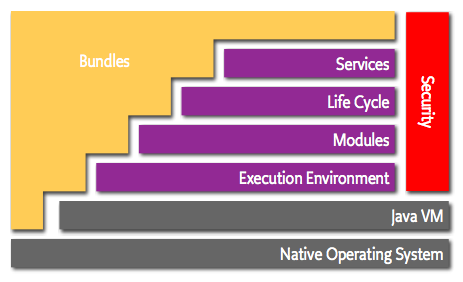
\includegraphics[scale=1.8]{figures/layering-osgi.png}
    \caption{From the official OSGI documentation\cite{osgiFrameworkArchitec22:online}.}
    \label{fig:osgiLayerModel}
\end{figure}
The Service layer interconnects the bundles makingit possible for them to communicate via plain old java objects (POJO).The Life-Cycle layer handles the the state of the application (start, stop, update and uninstall). The Modules layer defines how an application can import and export code and the Execution Environemnt defines which methods and classes are available in a specific environemnt. Finally, the Security layer encompases all other layers and handles for example code authentication, the digital signing of jar files, file access restrictions, certificates and more.\\
To the authors best knowledge there are currently six frameworks implementing the OSGi model. One such solution is the Bosch IoT Gateway Software\cite{BoschIoT13:online}. In a blog entry from 2015 Bosch compares the OSGi technology to other gateway solutions and says it "is the only one with clearly defined specs and an open specification process behind them"\cite{boschBlogOSGi69:online}. Boschs solution is proprietary and tailer made for edge-computing devices with IIoT in mind\cite{OSGiforIoTBlog27:online}. It runs on Linux, Windows, mac OS, Android, and VxWorks and according to Bosch more than 40 different gateway devices\cite{BoschIoT13:online}. The software is stable at major version 9 and still under heavy development. Because of these reasons, it is used as an examplary solution. \Cref{fig:boschIoTGatewaySetup} shows where Boschs IoT solution is situated in the IoT environment. Bosch provides the OSGi framework implementation for the gateways and additional features for the cloud to ease the management of the gateways and store the accumulated data.
\begin{figure}[h!]
    \centering
    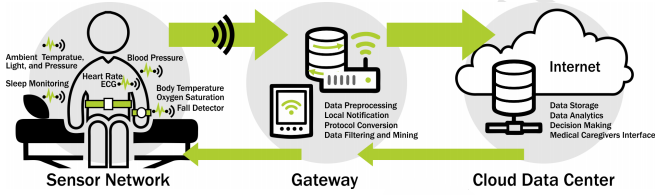
\includegraphics[scale=1.8]{figures/iotSetup.png}
    \caption{From the official Bosch documentation \cite{BoschIoT13:online}.}
    \label{fig:boschIoTGatewaySetup}
\end{figure}
A strong argument for this solution is the number of protocols it supports (BLE, ZigBee and MQTT, just to name a few) as well as its maturity.




\subsection{Disconnected Orchestrated Solutions}
IoT cluster solutions\\
Isolated k8s cluster: Solution k3s\\
Kubernetes cluster where edge is part of the cloud: kubeedge\\
% https://github.com/kubernetes/website/pull/13158



\subsection{Connected orchestrated solutions}
Edged: an agent that runs on edge nodes and manages containerized applications.
EdgeHub: a web socket client responsible for interacting with Cloud Service for the edge computing (like Edge Controller as in the KubeEdge Architecture). This includes syncing cloud-side resource updates to the edge, and reporting edge-side host and device status changes to the cloud.
CloudHub: a web socket server responsible for watching changes at the cloud side, caching and sending messages to EdgeHub.
EdgeController: an extended kubernetes controller which manages edge nodes and pods metadata so that the data can be targeted to a specific edge node.
EventBus: a MQTT client to interact with MQTT servers (mosquitto), offering publish and subscribe capabilities to other components.
ServiceBus: a HTTP client to interact with HTTP servers (REST), offering HTTP client capabilities to components of cloud to reach HTTP servers running at edge.
DeviceTwin: responsible for storing device status and syncing device status to the cloud. It also provides query interfaces for applications.
MetaManager: the message processor between edged and edgehub. It is also responsible for storing/retrieving metadata to/from a lightweight database (SQLite).

https://randomnerdtutorials.com/esp32-over-the-air-ota-programming/